\documentclass[16]{article} %[Tamaño de página y número de fuente]. %Tipo del documento
\usepackage{amsmath} %Añade comandos para ecuaciones
\usepackage[spanish]{babel} %Indica idioma del documento
\usepackage[utf8]{inputenc} %Permite escribir caracteres particulares del español (tildes, ñ, ...). Equivalente a poner \'a
\usepackage{vmargin} %Para editar márgenes
\usepackage{graphicx} %Permite instertar imágenes
\usepackage{tikz} %Permite insertar elementos gráficos
\usepackage[linesnumbered]{whilecode2} %Para escribir código en WHILE

\begin{document} %Crea el entorno del documento
\begin{titlepage} %Portada
	\centering  %Centra el texto
	{\bfseries\Huge Teoría de Autómatas y Lenguajes Formales\par}
   	\vspace{2cm} %Crea un espacio vertical
    {\bfseries\huge Actividades Práctica 3\par}
    \vfill %Rellena el espacio para ocupar la página entera
    {\huge Iván Romero Molina\par}
    \vspace{1cm}
    {\Large Universidad de Málaga\par}
    \vspace{1cm}
    {\large 26 de diciembre de 2022\par}
\end{titlepage}
    
\newpage
%\thispagestyle{empty} Quita el número de página
\section*{Actividad 1}	%Si tiene * quita la numeración
\noindent
Define una TM que sume dos número naturales y pruebe su funcionamiento.\\\\
Ejemplo 1 (suma 0+0):\\\\
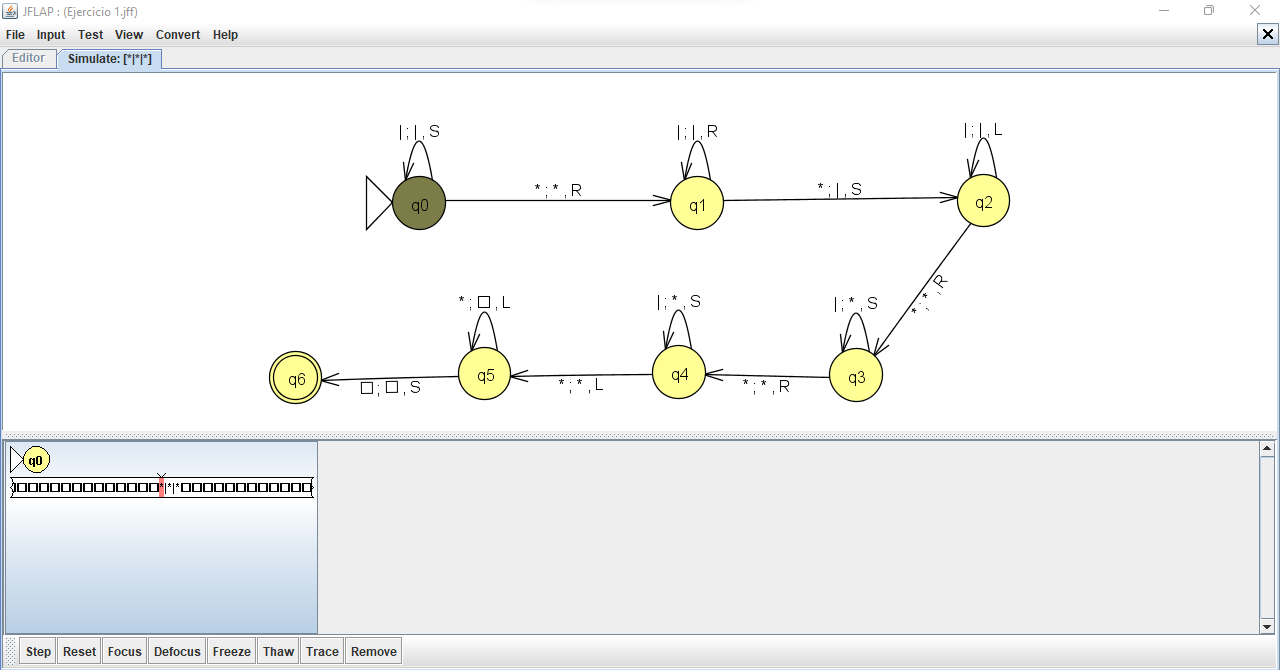
\includegraphics[width=1.1\linewidth]{Ejercicio1a.png}\\\\
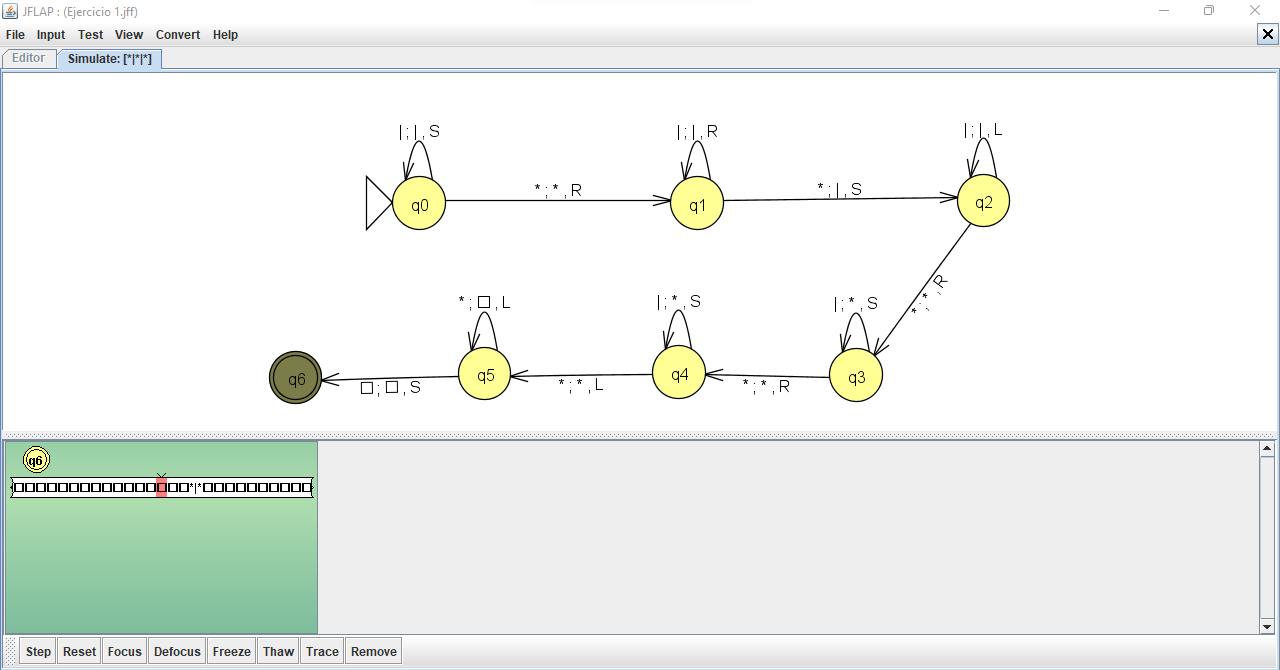
\includegraphics[width=1.1\linewidth]{Ejercicio1b.png}
\newpage
\noindent
Ejemplo 2 (suma 1+2):\\\\
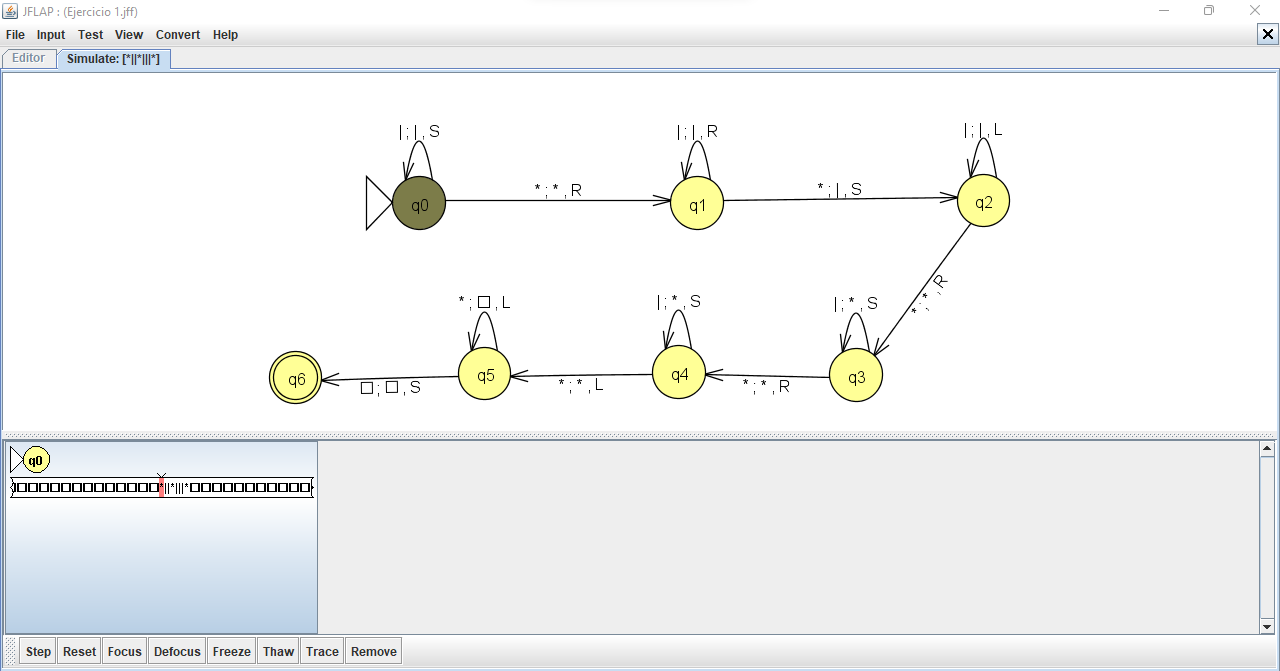
\includegraphics[width=1.1\linewidth]{Ejercicio1c.png}\\\\
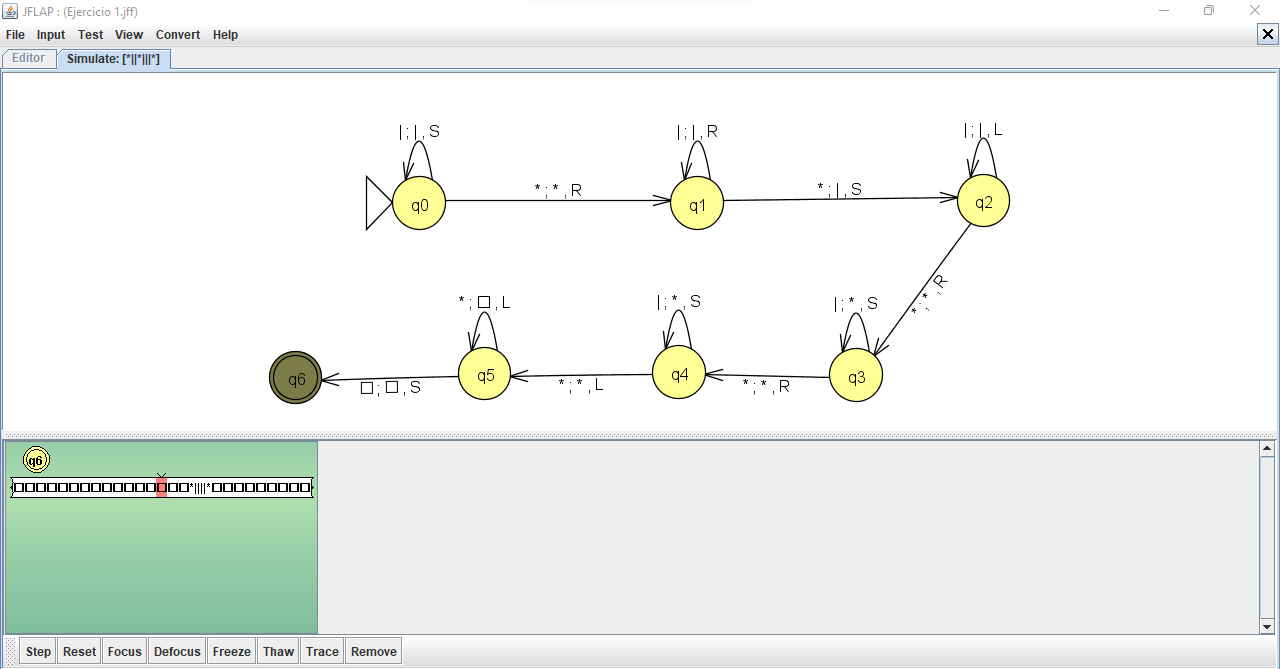
\includegraphics[width=1.1\linewidth]{Ejercicio1d.png}

\newpage
\section*{Ejercicio 2}
\noindent
Define una ecuación recursiva que sume tres valores (addition3):
\\\\
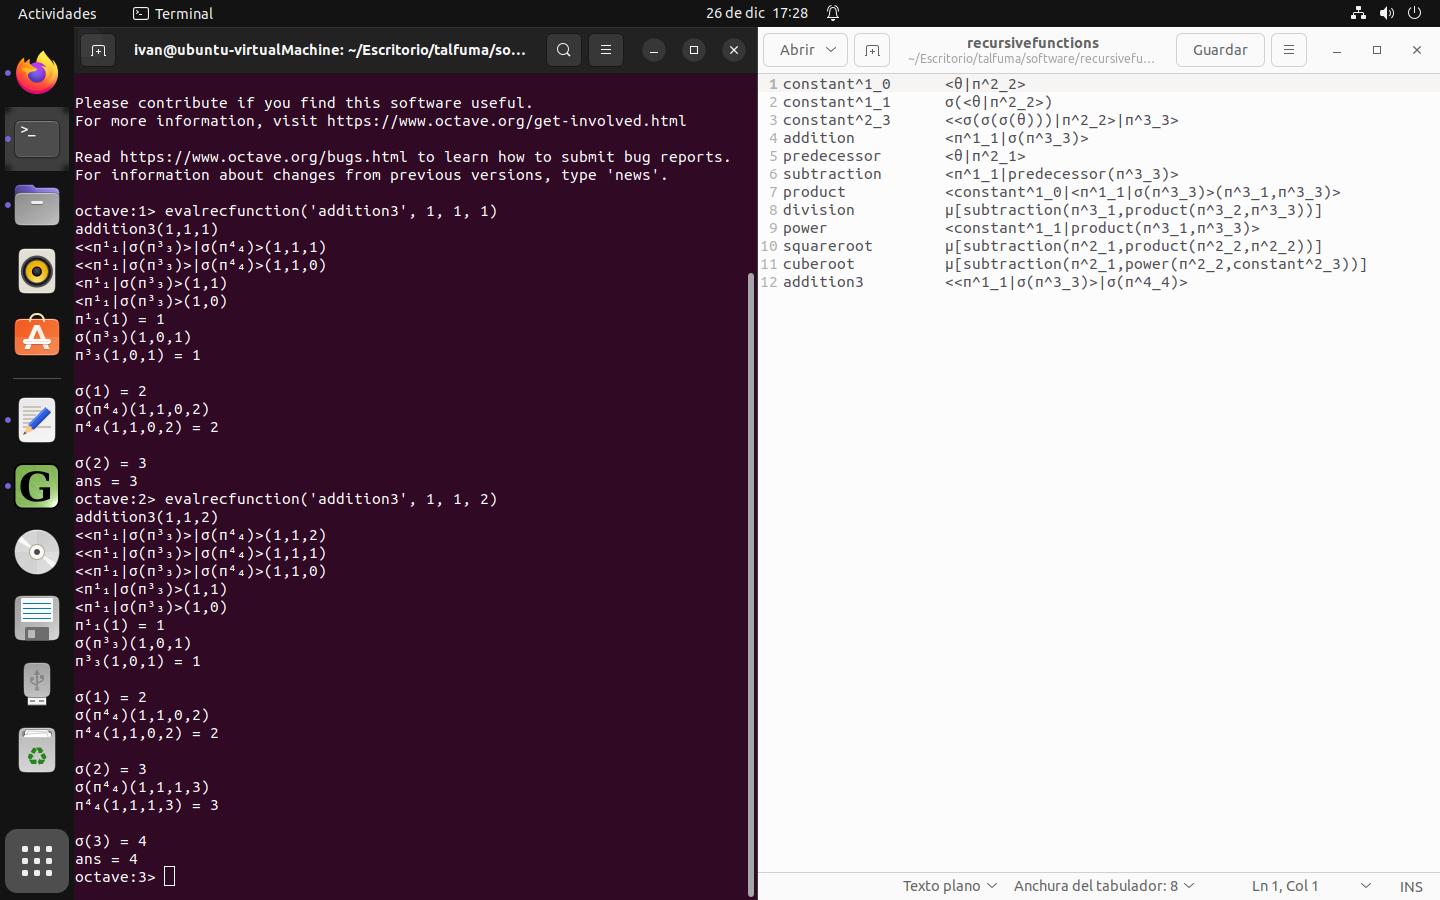
\includegraphics[width=1.1\linewidth]{Ejercicio2.png}

\newpage
\section*{Ejercicio 3}
\noindent
Implemente en un programa WHILE que realice la suma de tres valores, se debe usar una variable auxiliar que acumule el resultado de la suma.\\\\
Código en WHILE:
\whileprogram{suma}{3,4}{
\Copy{\Var{$X_4$}}{\Var{$X_1$}}
\WhileSC{\Var{$X_2$}$\neq0$}
{
	\Incr{\Var{$X_4$}}{1}
    \Decr*{\Var{$X_2$}}{1}
}
\WhileSC{\Var{$X_3$}$\neq0$}
{
	\Incr{\Var{$X_4$}}{1}
    \Decr*{\Var{$X_3$}}{1}
}
\Copy*{\Var{$X_1$}}{\Var{$X_4$}}
}{s}
\\\\
Ejemplo de una salida (1+1+1):\\\\
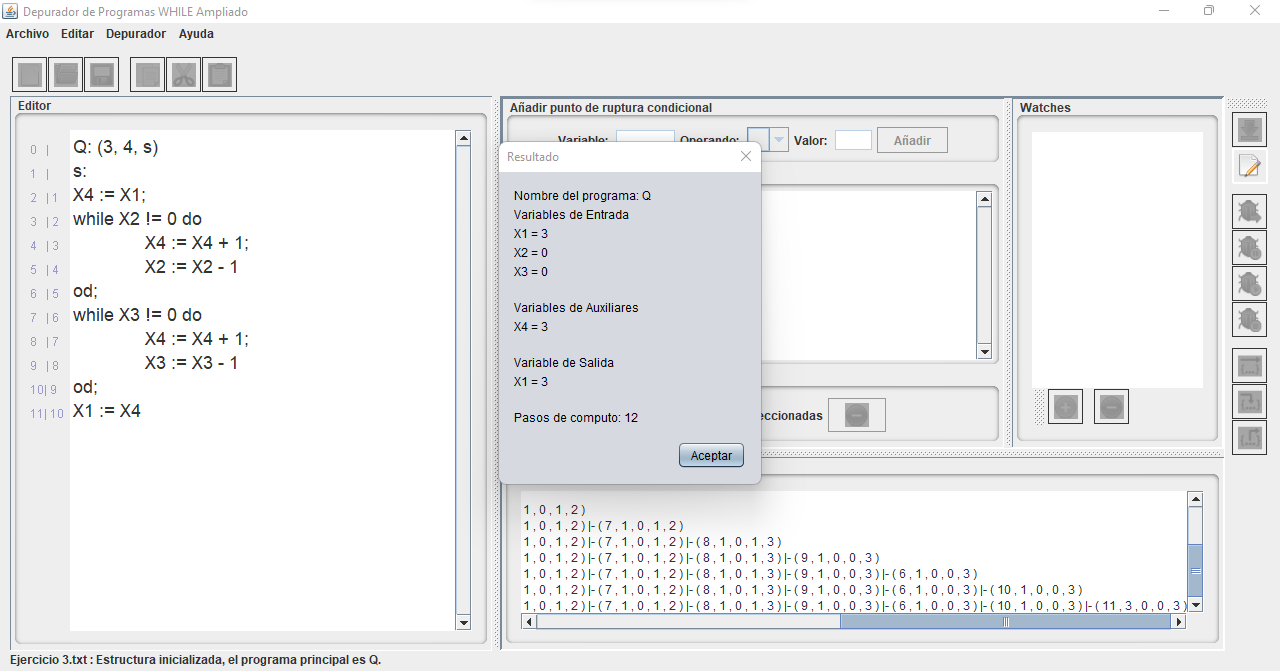
\includegraphics[width=1.1\linewidth]{Ejercicio3.png}
\end{document}